\begin{abstract}
%In this paper, we introduce several physical models of bowed and plucked string instruments based on accurate numerical simulations using finite-difference schemes (FDS), which are also efficient enough to run in real-time. We describe 
In this paper, implementation, instrument design and control issues surrounding a modular physical modelling synthesis environment are described. The environment is constructed as a network of stiff strings and a resonant plate, accompanied by user-defined connections and excitation models. The bow, in particular, is a novel feature in this setting. The system as a whole is simulated using finite difference (FD) methods. The mathematical formulation of these models is presented, alongside several new instrument designs, together with a real-time implementation in JUCE using FD methods. Control is through the Sensel Morph.  
\end{abstract}
%

\section{Introduction}\label{sec:introduction}

Physical models for sound synthesis have been researched for several decades to mathematically simulate the sonic behaviour of musical instruments and everyday sounds. Various techniques and methodologies have developed, ranging from mass-spring models \cite{cadoz79, Cadoz83, cadoz1993cordis} to modal synthesis \cite{morrison1993mosaic} and waveguide based models \cite{smith1992physical}. The latter two techniques may be viewed as numerical simulation techniques applied to the systems of partial differential equations (PDEs). These equations define the dynamics of a musical instrument, either real or imagined.

Mainstream time-domain simulation techniques, such as finite difference (FD) methods, were first applied to the case of string vibration by Ruiz \cite{Ruiz} and Hiller and Ruiz \cite{Hiller, Hiller2}, and then later by other authors \cite{Bacon} including, most notably Chaigne \cite{Chaigne92} and Chaigne and Askenfelt \cite{Chaigne}. The general use of finite-difference schemes (FDSs) in sound synthesis is described in \cite{Bilbao2009:NumericalSoundSynthesis}. Modularized physical modelling sound synthesis, whereby the user may construct a virtual instrument using basic canonical components dates back to the work of Cadoz and collaborators \cite{cadoz79, Cadoz83, cadoz1993cordis}. It has been also used as a design principle in the context of FD methods \cite{Bilbao2009:ModularPercussion, Bilbaosmc14, Webb2015}, where the canonical elements are strings and plates, with a non-linear connection mechanism.  Though computational cost of such methods is high, standard computing power is now approaching a level suitable for real-time performance for simpler systems.  

We are interested in bridging the gap between large-scale modular physical modelling synthesis and sonic interaction design \cite{franinovic2013sonic}, to be able to play with such simulations in real-time. Specifically, we are interested in using the expressivity of the Sensel Morph \cite{sensel2018} to control our simulations, using both percussive and bowing excitations. Our ultimate goal is to create models that are both mathematically accurate and efficient. This goal is nowadays possible thanks to improvements in hardware and software technologies for sound synthesis, yet it has rarely been achieved. The ultimate goal is to provide a modular efficient synthesizer based on accurate simulations, where real-time expressivity can also be achieved. This synthesizer has already been informally evaluated by composers and sound designers, who appreciated the current sonic palette.

% Used Modular Percussion Synthesis Environment (Bilbao) + On the limits of real-time physical modelling synthesis with a modular environment (Webb + Bilbao) as a basis and extended it to be interactive and used melodic rather than percussive components/elements.

This paper is structured as follows: Section \ref{sec:PDE} describes the physical models used in the implementation and Section \ref{sec:FDS} shows a general description of the FD methods used to digitally implement these models. Furthermore, Section \ref{sec:implementation} elaborates on the real-time implementation, Section \ref{sec:instruments} shows several different configurations of the physical models inspired by real musical instruments, Section \ref{sec:discussion} will present the results on CPU usage and evaluation and discuss this and finally, in Section \ref{sec:conclusion}, some concluding remarks appear.

\section{Models}\label{sec:PDE}
In this section, the PDEs for the damped stiff string and plate will be presented. The notation used will be the one found in \cite{Bilbao2009:NumericalSoundSynthesis} where the subscript for state variable $u$ denotes a single derivative with respect to time $t$ or space $x$ respectively. Furthermore, to simplify the presented physical models, non-dimensionalization (or scaling) will be used \cite{Bilbao2009:NumericalSoundSynthesis}. 

% \begin{equation}
%     \pdv[2]{u}{t} = \gamma^2 \pdv[2]{u}{x} -\kappa^2 \pdv[4]{u}{x} - 2\sigma_0\pdv{u}{t} + 2\sigma_1\frac{\partial^3u}{\partial tx^2}
% \end{equation}

\subsection{Stiff string}\label{subsec:stiffStringPDE}
A basic model of the linear transverse motion of a string of circular cross section may be described in terms of several parameters: the total length $L$ (in m), the material density $\rho$ (in kg$\cdot$m$^{-3}$), string radius $r$ (in m), Young's modulus $E$ (in Pa), tension $T$ (in N), and two loss parameters $\sigma_{0}$ and $\sigma_{1}$. %, to be described shortly.
The PDE for a damped stiff string may be written as
    \cite{Bilbao2009:NumericalSoundSynthesis} 
\begin{equation}\label{eq:stiffString}
    u_{tt} = \gamma^2 u_{xx}-\kappa^2u_{xxxx} - 2\sigma_0u_{t} + 2\sigma_1u_{txx}.
\end{equation}
In this representation, spatial scaling has been employed using a length $L$, so the solution $u = u(x,t)$ is defined for $t\geq 0$ and for dimensionless coordinate $x\in[0,1]$. Furthermore, parameters $\gamma = \sqrt{T/\rho\pi r^2 L^2}$ and $\kappa = \sqrt{Er^2/4\rho L^4}$ and have units s$^{-1}$.% Subscripts represent partial differentiation with respect to time $t$ and coordinate $x$. 

In this work, the string is assumed clamped at both ends, so that
\begin{equation}\label{boundary}
    u = u_x = 0 \quad \text{where} \quad x = \{0, 1\}.
\end{equation}
A model of a bowed string \cite{Bilbao2009:NumericalSoundSynthesis} may be incorporated into \eqref{eq:stiffString} as  
\begin{subequations}
\begin{align}
    \label{eq:bowedString} &u_{tt} = \hdots - \delta(x-x_\text{B})F_\text{B}\phi(v_\text{rel}), \quad \text{with} \\
    &v_\text{rel} = u_t |_{(x = x_\text{B})} - v_\text{B},\label{eq:relVelocity}
\end{align}
\end{subequations}
%the $\delta$ function is only non-zero at the bowing point, effectively locating the bowing interaction.  
where $F_\text{B} = f_\text{B}/ M_\text{s}$ is the excitation function (in m/s$^2$) with externally-supplied bowing force $f_\text{B} = f_\text{B}(t)$ (in N) and total string mass $M_\text{s} = \rho\pi r^2 L$ (in kg). The relative velocity $v_\text{rel}$ is defined as the difference between the velocity of the string at bowing point $x_\text{B}$ and the externally-supplied bowing velocity $v_\text{B} = v_\text{B}(t)$ (in m/s) and $\phi$ is a dimensionless friction characteristic, chosen here as \cite{Bilbao2009:NumericalSoundSynthesis}
\begin{equation}
    \phi(v_\text{rel}) = \sqrt{2a}v_\text{rel} e^{-av_\text{rel}^2+1/2}.
\end{equation}
Furthermore, $\delta(x-x_\text{B})$ is a spatial Dirac delta function selecting the bowing location $x=x_\text{B}$. The single bowing point can be extended to a bowing area \cite{Bilbao2009:NumericalSoundSynthesis}. More detailed models of string dynamics, again in a bowed string context, have been proposed by Desvages \cite{Desvages16}. 

Another, and more simple way to excite the string is by extending Equation \eqref{eq:stiffString} to
\begin{equation}
    \label{eq:excitedString} u_{tt} = \hdots + E_\text{e}F_\text{e}%,
\end{equation}
using an externally-supplied distribution function $E_\text{e} = E_\text{e}(x)$ and excitation function $F_\text{e} = F_\text{e}(t)$. In this case, the excitation region is allowed to be of finite width.

\subsection{Plate}\label{subsec:platePDE}
Under linear conditions, a rectangular plate of dimensions $L_{x}$ and $L_{y}$ may be parameterized in terms of density $\rho$ (in kg$\cdot$ m$^{-3}$), thickness $H$ (in m), Young's modulus $E$ (in Pa) and a dimensionless Poisson's ratio $\nu$, as well as two loss parameters $\sigma_{0}$ and $\sigma_{1}$.%, to be discussed shortly.  

In terms of dimensionless spatial coordinates $x$ and $y$ scaled by $\sqrt{L_{x}L_{y}}$, the equation of motion of a damped plate is a variant of the Kirchhoff model \cite{Graff}
\begin{equation}\label{eq:platePDE}
    u_{tt} = -\kappa^2 \Delta\Delta u - 2 \sigma_0 u_{t} + 2\sigma_1 \Delta u_{t}.
\end{equation}
Here, $u(x,y,t)$ is the transverse displacement of the plate as a function of dimensionless coordinates $x\in[0, \sqrt{a}\,]$, $y\in[0,1/\sqrt{a}\,]$, where $a = L_{x}/L_{y}$ is the plate aspect ratio, as well as time $t$. Furthermore, $\Delta$ represents the 2D Laplacian \cite{Bilbao2009:NumericalSoundSynthesis}:
\begin{equation}
    \Delta  = \frac{\partial^2}{\partial x^2}+\frac{\partial^2}{\partial y^2}.
\end{equation}
The stiffness parameter $\kappa$, with dimensions of s$^{-1}$, is defined by $\kappa = \sqrt{D/\rho H L_{x}^2L_{y}^2}$ where $D = EH^3/12\left(1-\nu^2\right)$. As in the case of the stiff string, we chose to use clamped boundary conditions:
\begin{equation}
        u = {\bf n}\cdot \nabla u = 0 
\end{equation}
over any plate edge with outward normal direction ${\bf n}$ and where $\nabla u$ is the gradient of $u$. 
%need to explain subscript y?
\subsection{Connections}\label{sec:connections}
Adding connections between different physical models, further referred to as elements, adds another term to Equation \eqref{eq:bowedString}, \eqref{eq:excitedString} or \eqref{eq:platePDE}. Assuming that element $\alpha$ is a stiff string and $\beta$ is a plate, the following terms are added to the aforementioned equations:
%Equations \eqref{eq:bowedString}, \eqref{eq:excitedString} for bowed or simply excited strings or \eqref{eq:platePDE} for plates respectively:
%% this paragraph is too wide for some reason
\begin{subequations}
\begin{align}
    \label{eq:stringConnection}
    u_{tt} &= ... + E_{\text{c},\alpha}F_\alpha, \\
    \label{eq:plateConnection}
    u_{tt} &= ... + E_{\text{c},\beta}F_\beta,
\end{align}
\end{subequations}
with force-functions $F_\alpha = F_\alpha(t)$ and $F_\beta = F_\beta(t)$ (in m/s$^2$) and distribution functions $E_{\text{c},\alpha}$ and $E_{\text{c},\beta}$ which have chosen to be highly localised in our application and reduce to $\delta(x-x_{\text{c},\alpha})$ and $\delta(x-x_{\text{c},\beta}, y-y_{\text{c},\beta})$ respectively, but can be extended to be connection areas \cite{Bilbao2009:ModularPercussion}. We use the implementation as presented in \cite{Bilbao2009:ModularPercussion} where the connection between two elements is a non-linear spring. The forces it imposes on the elements it connects are defined as
\begin{subequations}\label{eq:connectionsPDE}
\begin{align}
    F_\alpha &= -\omega_0^2\eta - \omega_1^4\eta^3 - 2\sigma_\times\dot\eta,\\
    \label{eq:FBeta} F_\beta &= -\mathcal{M}F_\alpha,
\end{align}
\end{subequations}
where $\omega_0$ and $\omega_1$ are the linear (in s$^{-1}$) and non-linear (in $($m$\cdot$s$)^{-1/2}$) frequencies of oscillation respectively, $\sigma_\times$ is a damping factor (in s$^{-1}$), $\mathcal{M}$ is the mass ratio between the two elements and $\eta$ is the relative displacement between the connected elements at the point of connection (in m). Lastly, the dot above $\eta$ denotes a derivative with respect to time.

\section{Finite-Difference Schemes}\label{sec:FDS}
To be able to digitally implement the continuous equations shown in the previous section, they need to be approximated. In this section, a high-level review of a finite difference approximation to a connected system of strings and plates is presented. For more technical details, see \cite{Bilbao2009:ModularPercussion}. 

In the case of the stiff string, state variable $u(x,t)$ can be discretised at times $t = nk$, where $n \in \mathbb{N}$ and $k = 1 / f_\text{s}$ is the time step (at sample-rate $f_\text{s}$) and locations $x = lh$, with $l \in [0,\hdots, N]$ where the total number of points is $N+1$ and grid spacing $h$. We can now write the discretised state variable as $u_l^n$, representing an approximation to $u(x,t)$. 

In the case of the plate, $u(x,y,t)$ is discretised to $u_{(l,m)}^n$ using $x = lh$ where $l \in [0,\hdots, N_x]$ with $N_x+1$ being the total horizontal number of points and $y = mh$ where $m \in [0,\hdots,N_y]$ with $N_y+1$ being the total vertical number of points. 
%Approximations for the derivatives in the equations found in Section \ref{sec:PDE} can be found in \cite{Bilbao2009:NumericalSoundSynthesis}. 
%We will also use the notation for the difference and averaging operators found here. 

In a general sense, when discretising PDEs as presented in Equations \eqref{eq:stiffString} and \eqref{eq:platePDE}, we will need to solve for $\mathbf{u}^{n+1}$, i.e., $\mathbf{u}$ at the next time step, where $\mathbf{u}$ is a vector of size $N-1$ containing values of $u_l \ \forall l$ for a string and $(N_x-1)(N_y-1)$ containing values of $u_{(l,m)}\ \forall (l,m)$ for a plate. Note that the vector sizes are smaller than the total number of grid points as we do not include the values at the boundaries (which are always 0).
%$\mathbf{u}$ is a column vector of size $N-1$ containing values of $u$ at the appropriate time step
For a PDE expressed as a function of $u_{tt}$, its FDS will be of the form
\begin{equation}\label{eq:FDSform}
    \mathbf{u}^{n+1} = 2\mathbf{u}^n-\mathbf{u}^{n-1} + K\mathbfcal{F}^n,
\end{equation}
where
\begin{equation}\label{eq:K}
    K = \frac{k^2}{1+\sigma_0k},
\end{equation}
% \end{subequations}
and $\mathbfcal{F}^n$ is a combination of the discretised PDE (excluding terms containing $u^{n+1}$) together with connection and excitation terms.

\subsection{Stiff String}
In the case of the stiff string, $\mathbfcal{F}^n$ in Equation \eqref{eq:FDSform} is a combination of the discretised PDE \eqref{eq:stiffString} $\mathbf{f}_\alpha^n$, connection term \eqref{eq:stringConnection} and bowing \eqref{eq:bowedString}
\begin{subequations}
\begin{equation}\label{eq:FDSbowedString}
\mathbfcal{F}^n = \mathbf{f}_\alpha^n + \mathbf{E}_{\text{c},\alpha}F_\alpha^n - \mathbf{J}(x_\text{B}^n)F_\text{B}^n\phi(v_\text{rel}),
\end{equation}
or excitation \eqref{eq:excitedString} term
\begin{equation}\label{eq:FDSexcitedString}
    \mathbfcal{F}^n = \mathbf{f}_\alpha^n + \mathbf{E}_{\text{c},\alpha}F_\alpha^n + \mathbf{E}_\text{e}F_\text{e}^n,% \quad \quad \ \ \;\,
\end{equation}
\end{subequations}
where $\mathbf{E}_{\text{c},\alpha}$ contains the discretised distribution function for the connection ($1/h$ at connection index $l_{\text{c},\alpha}$, rest 0's \cite{Bilbao2009:NumericalSoundSynthesis}), $\mathbf{E}_\text{e}$ contains the discretised distribution function for the excitation (which will be presented in Equation \eqref{eq:discDist} in the next section) and $\mathbf{J}(x_\text{B}^n)$ is a spreading operator containing the discretised bowing distribution ($1/h$ at time-varying bowing position $x_\text{B}$). If $x_\text{B}$ is between grid points, cubic interpolation is used to spread the bow-force over neighbouring grid points \cite{Bilbao2009:NumericalSoundSynthesis}. All vectors are columns of size $N - 1$. 

It can be useful to talk about the \textit{region of operation} of a FDS in terms of a `stencil'. A stencil describes the number of grid points needed to calculate a single point at the next time step. The stiff string FDS has a stencil of 5 grid points. In other words, two grid points at either side of $l$ -- and $l$ itself -- are necessary to calculate $u^{n+1}_l$. See Figure \ref{fig:stencil1D} for a visualisation of this.
\begin{figure}[ht]
    \centering
    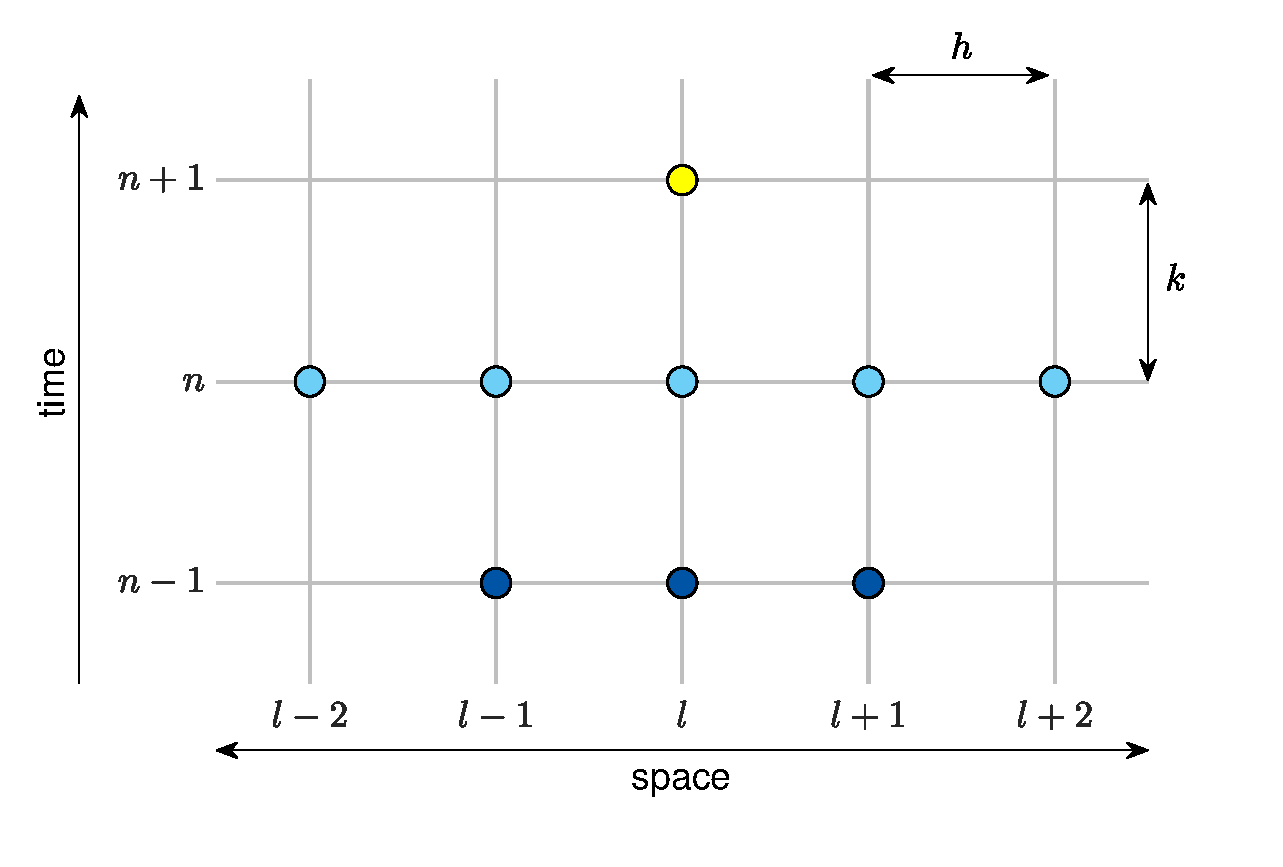
\includegraphics[width=\paperFigWidth\textwidth]{figures/stencil1Dedit.eps}
\caption{Stencil for a stiff string FDS with grid spacing $h$ and time step $k$. The point $l$ at the next time step (yellow) is calculated using 5 points at the current time step (blue) and 3 at the previous time step (dark blue). \label{fig:stencil1D}}
\end{figure}

In order for the scheme to be stable, the grid spacing needs to abide the following condition \cite{Bilbao2009:NumericalSoundSynthesis}
%section 7.2.3 numerical sound synthesis
\begin{equation}\label{eq:stabilityString}
    h \geq \sqrt{\frac{\gamma^2 k^2 + 4 \sigma_1 k + \sqrt {(\gamma^2 k^2 + 4 \sigma_1 k)^2 + 16 \kappa^2 k^2}}{2}}.
\end{equation}
The closer $h$ is to this limit, the higher the quality of the implementation. The number of points $N$ can then be calculated using 
\begin{equation}\label{eq:NString}
    N = \text{floor}\bigg(\frac{1}{h}\bigg).
\end{equation}

%\textit{Note: In this paper we have used the simple case of a single point for bowing and connections. These can be extended to a bowing area or area of connection. For more information on this, we would like to refer the reader to \cite{Bilbao2009:NumericalSoundSynthesis} for bowing area and \cite{Bilbao2009:ModularPercussion} for area of connection}.
\subsection{Plate}
In the case of the plate, $\mathbf{u}$ is a column vector of concatenated vertical `strips' of the plate state as in \cite{Bilbao2009:ModularPercussion} of size $(N_x-1)(N_y-1)$ and $\mathbfcal{F}^n$ in Equation \eqref{eq:FDSform} is a combination of the discretised PDE \eqref{eq:platePDE} $\mathbf{f}_\beta^n$ and connection term \eqref{eq:plateConnection}
\begin{equation}\label{eq:FDSplate}
    \mathbfcal{F}^n = \mathbf{f}_\beta^n + \mathbf{E}_{\text{c},\beta}F_\beta^n.
\end{equation}
Here, $\mathbf{E}_{\text{c},\beta}$ contains the discretised distribution function for the connection ($1/h^2$ at connection index ($l_{\text{c},\beta}$, $m_{\text{c},\beta}$), rest 0's \cite{Bilbao2009:ModularPercussion}) and is a column vector of size $(N_x-1)(N_y-1)$.
%OR SHOULD I ADD ",\alpha" OR ",\beta" TO l_c
For the plate, the stencil will consist of 13 grid points as can be seen in Figure \ref{fig:stencil2D}.
\begin{figure}[h]
\centering
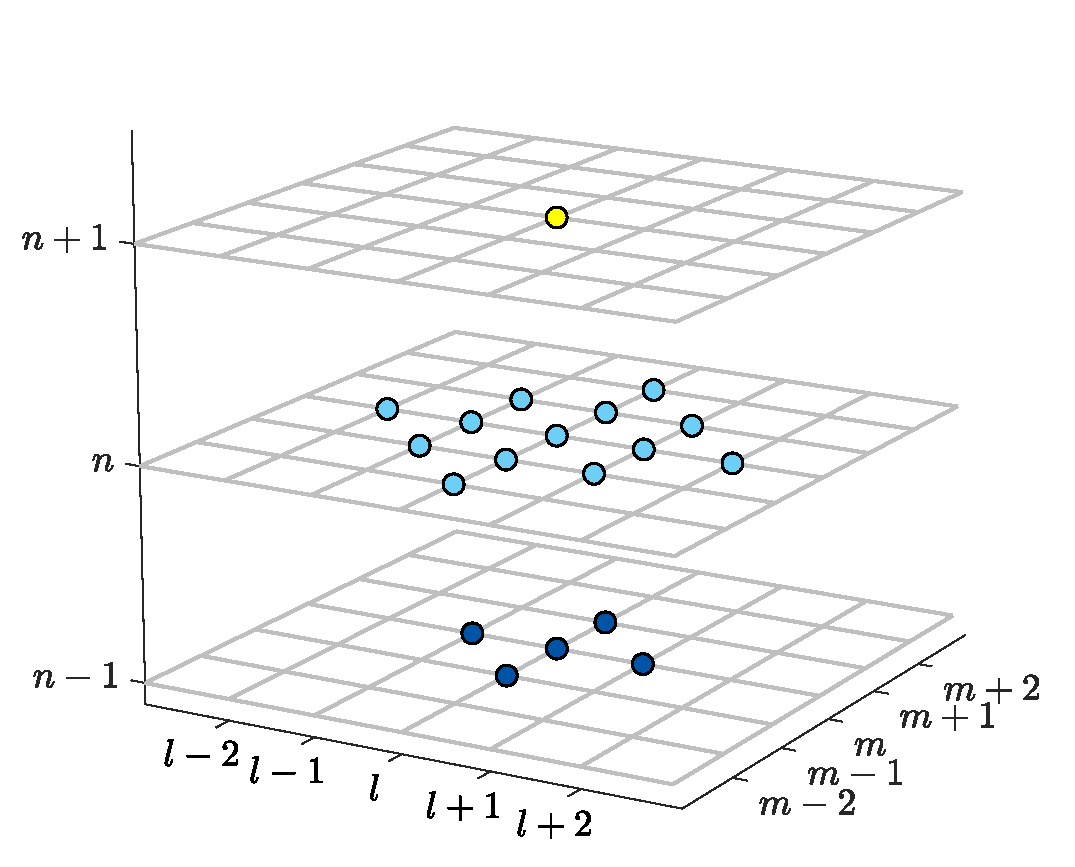
\includegraphics[width=\paperFigWidth\textwidth]{figures/stencil2Dedit.eps}
\caption{Stencil for a plate FDS. The point $(l,m)$ at the next time step (yellow) is calculated using 13 points at the current time step (blue) and 5 at the previous time step (dark blue). \label{fig:stencil2D}}
\end{figure}

\noindent The grid spacing needs to abide the following condition \cite{Bilbao2009:ModularPercussion}
\begin{equation}\label{eq:stabilityPlate}
h \geq 2\sqrt{k\bigg(\sigma_1^2 + \sqrt{\kappa^2+ \sigma_1^2}\bigg)},
\end{equation}
(again, the closer $h$ is to this limit the better) from which $N_x$ and $N_y$ can be derived using
\begin{equation}
    N_x = \text{floor}\Bigg(\frac{\sqrt{a}}{h}\Bigg) \quad \text{and} \quad
    N_y = \text{floor}\Bigg(\frac{1}{h\sqrt{a}}\Bigg).
\end{equation}

\subsection{Connections}
In the following, we discretise the equations in \eqref{eq:connectionsPDE} as shown in \cite{Bilbao2009:ModularPercussion}. However, as these equations are not expressed as a function of $u_{tt}$, their FDS counterpart will be different. Moreover, instead of solving for $\mathbf{u}^{n+1}$, we need to solve for $\eta^{n+1}$, i.e., the relative displacement at the next time step, which will be in the form of
\begin{equation}\label{eq:etaNext}
    \eta^{n+1} = p^nF_\alpha^n + r^n\eta^{n-1},
\end{equation}
where $p^n = p(\eta^n)$ and $r^n = r(\eta^n)$ are functions of the relative displacement $\eta$ if $\omega_1 \neq 0$ and constants if $\omega_1 = 0$. Again, assuming that element $\alpha$ is a stiff string and $\beta$ is a plate, $\eta$ can be calculated using
\begin{equation}\label{eq:relativeDisp}
    \eta^n = h_\alpha u_{\alpha, l_{\text{c},\alpha}}^n - h_\beta^2 u_{\beta,(l_{\text{c},\beta}, m_{\text{c},\beta})}^n.
\end{equation}
In other words, this is the difference between the state of element $\alpha$ at $l_{\text{c},\alpha}$ and the state of element $\beta$ at $(l_{\text{c},\beta}, m_{\text{c},\beta})$ scaled by their respective (for plates, squared) grid spacings $h_\alpha$ and $h_\beta$. %It is important to note that this can only be done when the connection is a point rather than an area, in which case an inner product needs to be taken over the  
The next step is to obtain $F^n_\alpha$, which can be used to easily calculate $F^n_\beta$. We first obtain values for $\mathbf{u}^{n+1}$ by solving \eqref{eq:FDSform} using \eqref{eq:FDSbowedString}, \eqref{eq:FDSexcitedString} or \eqref{eq:FDSplate} (without the connection term!) for a string or plate respectively. As, at this point, no connection forces have been added yet, this state will be referred to as an intermediate state $\mathbf{u}^\text{I}$. This intermediate state can be used to obtain $\eta^{n+1}$ using \eqref{eq:relativeDisp}
\begin{equation}
% \begin{aligned}
    \eta^{n+1} = h_\alpha( u_{\alpha,l_{\text{c},\alpha}}^\text{I} + K_\alpha F^n_\alpha) - \Big[h^2_\beta( u_{\beta,(l_{\text{c},\beta}, m_{\text{c},\beta})}^\text{I} 
    + K_\beta F^n_\beta)\Big],
% \end{aligned}
\end{equation}
where $K_\alpha$ and $K_\beta$ are as described in \eqref{eq:K} using the damping coefficient $\sigma_0$ of their respective element. This can then be set equal to \eqref{eq:etaNext}. Using Equation \eqref{eq:FBeta}, solving for $F_\alpha$ yields
\begin{equation}
    F_\alpha^n = \frac{r^n\eta^{n-1}-(h_\alpha u_{\alpha, l_{\text{c},\alpha}}^\text{I} - h^2_\beta u_{\beta,(l_{\text{c},\beta},m_{\text{c},\beta})}^\text{I})}{h_\alpha K_\alpha + \mathcal{M}h^2_\beta K_\beta-p^n}.
\end{equation}
% where $K$ for element E is defined as
% \begin{equation}
%     K_\text{E} = \frac{k^2}{1+\sigma_{0,\text{E}}k}.
% \end{equation}

% This scaling factor is also used when adding the connection forces to the state $u$ where FDSs \eqref{eq:bowedStringFDS} and \eqref{eq:plateFDS} are extended to:
% \begin{equation}
% \begin{aligned}
%     \delta_{tt}u_l^n &= ... + J_\alpha F_\alpha E_\alpha\ ,\\
%     \delta_{tt}u_l^n &= ... + J_\beta F_\beta E_\beta\ .
% \end{aligned}
% \end{equation}
\section{Implementation}\label{sec:implementation}
%kind of a methods section 
% implementation of FDSs and C++ optimization
In this section, we elaborate more on the chosen values for the parameters described in the previous two sections and present the system architecture of the real-time application. The values for most parameters have been arbitrarily chosen and can -- as long as they satisfy the conditions in Equations \eqref{eq:stabilityString} and \eqref{eq:stabilityPlate} -- be changed. We used C++ along with the JUCE framework \cite{JUCE2019} for implementing the physical models and connections in real-time. The main hardware used was a MacBook Pro with a 2.2 GHz Intel Core i7 processor.

\subsection{Stiff String}
%In order to implement the FDSs presented in Section \ref{sec:FDS} they need to be solved for $u^{n+1}$. Equation \eqref{eq:stringImplementation} found in Appendix A shows a solved finite-difference scheme of Equation \eqref{eq:stiffStringFDS}.

As many string properties stay constant, we chose to set the following parameters directly, rather than calculating them from their physical properties: $
\kappa = 2$, $\sigma_0 = 1$, $\sigma_1 = 0.005$. An interesting parameter to make dynamic is the fundamental frequency $f_0$ (in s$^{-1}$) of the string. According to \cite{Bilbao2009:NumericalSoundSynthesis}, the fundamental frequency can be approximately calculated using
\begin{equation}
    f_0 \approx \frac{\gamma}{2}.
\end{equation}
However, as the grid spacing $h$ is dependent on the wave speed $\gamma$ according to the condition found in \eqref{eq:stabilityString}, we must put a lower limit on the number of points $N$ if we plan to dynamically increase $\gamma$.
%maybe it would be better to move the boundary to a different gridpoint and use interpolation for determination of the values around the boundary

Another way to change frequency is to add damping to the model at specific points acting as a (simplified) fretting finger. The advantage of this is that the condition \eqref{eq:stabilityString} will never be violated. On top of this, a tapping sound will be introduced when fretting the string making it more realistic than changing the wave speed. If the string is fretted at single location $x_\text{f} \in [0, 1]$ and $l_\text{f} = \text{floor}(x_\text{f}/h)$ we use
\begin{equation}
u_l^n = 
    \begin{cases}
        \hfil 0, & l = l_\text{f} - 1 \vee l = l_\text{f}\\
        \hfil (1-\alpha_\text{f}^\epsilon) u_l^n, & l = l_\text{f} + 1\\
        \hfil u_l^n, & \text{otherwise}
    \end{cases}
\end{equation}
where $\alpha_\text{f} = x_\text{f}/h - l_\text{f}$ describes the fractional location of $x_\text{f}$ between two grid points. Note that the grid point at the finger location and the grid point before are set to 0 to (recalling the stencil) prevent the states at either side of the finger to influence each other. The disadvantage of using this technique over regular linear interpolation, is that the effect of damping between grid points does not linearly scale to pitch. We thus added $\epsilon = 7$ as a heuristic value to more properly map finger position to pitch.

In some cases, $N$ is fixed to a certain value (as opposed to calculating it from Equations \eqref{eq:stabilityString} and \eqref{eq:NString}) for multiple strings of different pitches. Even though some bandwidth will be lost (in the higher frequency range), this will allow the strings to be perfectly tuned to each other.

\subsubsection{Bowed String}
Parameters for the bowed strings abide the following conditions: $|v_\text{B}| \leq 1$ m/s and $0 \leq F_\text{B} \leq 100$ N. It was chosen to discretise Equation \eqref{eq:relVelocity} implicitly %(STEFAN?)
making it necessary to use an iterative root-finding method such as Newton-Raphson \cite{Wallis1685}.

\subsubsection{Excited string}
If simply excited, we set the distribution function to a raised cosine with width $w_\text{e}$ (in grid points)
%% Continuous version
% \begin{equation} \label{eq:distribution}
%     E(x) = 
%     \begin{cases}
%         \hfil \frac{1 - \cos(\frac{2 \pi (x - x_\text{e})}{w_\text{e}})}{2}, & x_\text{e} -  \frac{w_\text{e}}{2} \leq x \leq x_\text{e} + \frac{w_\text{e}}{2} \\
%         \hfil 0, &\text{otherwise}
%     \end{cases}
% \end{equation}
% scaled by the excitation function over time with excitation duration $d_\text{e}$ [s]
% %numerical sound synthesis Eq. (12.28) or
% %On the limits of Eq. (4)
% \begin{equation}\label{eq:excitation}
%     F(t) = 
%     \begin{cases}
%         f_\text{e}\frac{1 - \cos(\frac{\pi (t - t_\text{e})}{d_\text{e}})}{2}, & t_\text{e} \leq t \leq t_\text{e}+d_\text{e}\\
%         \hfil 0, &\text{otherwise}
%     \end{cases}
% \end{equation}
% with excitation force $f_\text{e}$ [N]. 
% The distribution function is set to a raised cosine with width $w_\text{e}$

%% Discretised version
\begin{equation}\label{eq:discDist}
    E_\text{e}(l) = 
    \begin{cases}
        \hfil \frac{1 - \cos(\frac{2 \pi (l - (l_\text{e}-w_\text{e}/2))}{w_\text{e}})}{2}, & l_\text{e} -  \frac{w_\text{e}}{2} < l < l_\text{e} + \frac{w_\text{e}}{2} \\
        \hfil 0, &\text{otherwise}
    \end{cases}
\end{equation}
scaled by the excitation function over time with excitation duration $d_\text{e}$ (in samples)
\begin{equation}\label{eq:discExcitation}
    F_\text{e}(n) = 
    \begin{cases}
        \frac{1 - \cos(\frac{\pi (n - n_\text{e})}{d_\text{e}})}{2}, & n_\text{e} \leq n < n_\text{e}+d_\text{e}\\
        \hfil 0, &\text{otherwise}
    \end{cases}
\end{equation}
A visualisation of this can be found in Figure \ref{fig:exctiation}.

\begin{figure}[h]
\centering
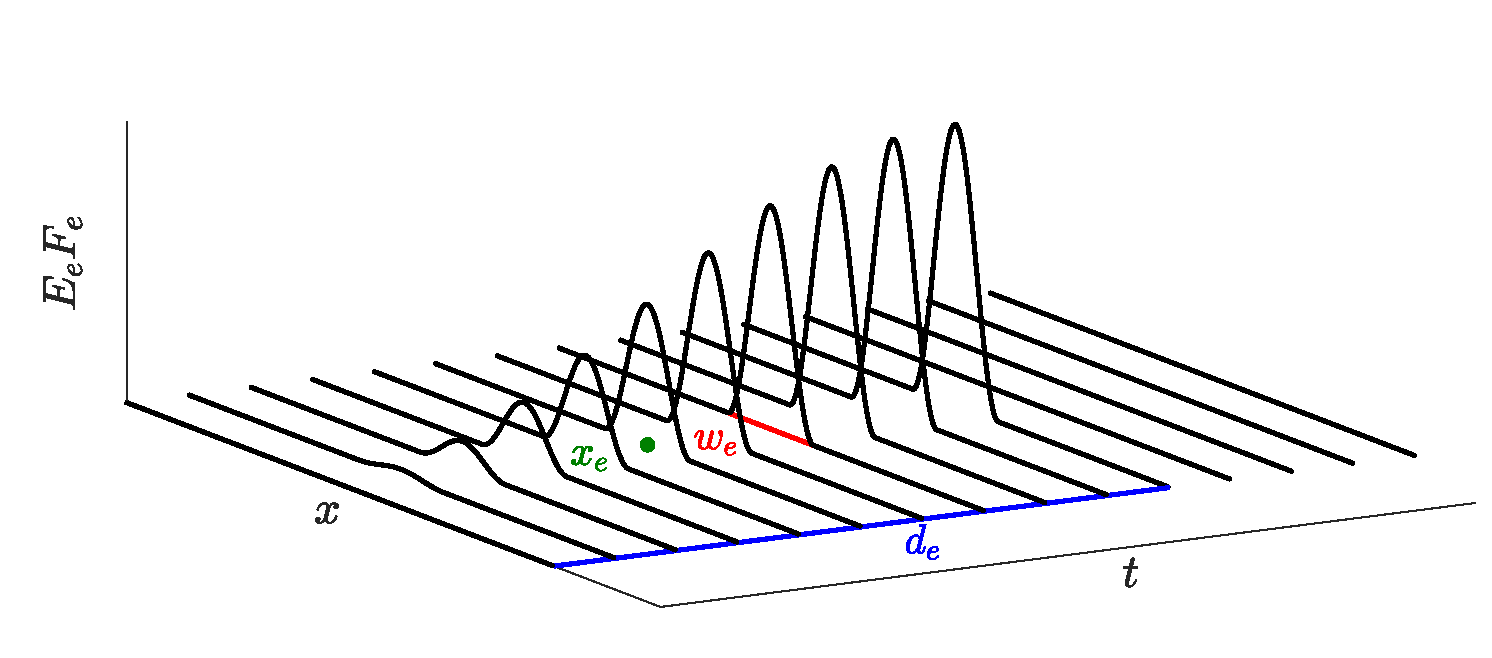
\includegraphics[width=\paperFigWidth\textwidth]{figures/excitation2.eps}
\caption{A visualisation of the excitation used in our implementation presented in Equation \eqref{eq:excitedString}. The location of excitation $x_\text{e}$ is shown in green, excitation width $w_\text{e}$ in red and excitation duration $d_\text{e}$ in blue (also see Equations \eqref{eq:discDist} and \eqref{eq:discExcitation}). \label{fig:exctiation}}
\end{figure}

\subsection{Plate}
For the plate, the damping coefficients have been decided to be $\sigma_0 = 0.1$ and $\sigma_1 = 0.005$ and the aspect ratio is set to $a = 2$. The plate stiffness $\kappa$ has been left as a user parameter to be changed dynamically and will be between the following bounds: $0.1 \leq \kappa \leq 50$ s$^{-1}$. In Equation \eqref{eq:stabilityPlate}, the grid spacing is calculated using the maximum value of $\kappa$ to prevent stability issues. Using a sample rate of 44,100 Hz results in a plate with dimensions $N_x = 20$ and $N_y = 10$ (in grid points).

\subsection{Connections}
Increasing $\omega_1 \gtrsim 100,000$ $($m$\cdot$s$)^{-1/2}$ while keeping $0 < \omega_0 \lesssim 100$ s$^{-1}$ will cause audible non-linear behaviour, such as pitch-glides and rattling sounds. These effects will be more dominant when the plate stiffness is higher. %string resonances?
In our implementation we set $\omega_0=100$ s$^{-1}$ and $\omega_1 = 100,000$ $($m$\cdot$s$)^{-1/2}$. The spring-damping $\sigma_\times = 1$ s$^{-1}$ is kept to a minimum ($0 \leq \sigma_\times \leq 10$ s$^{-1}$). 

\begin{figure}[h]
\centering
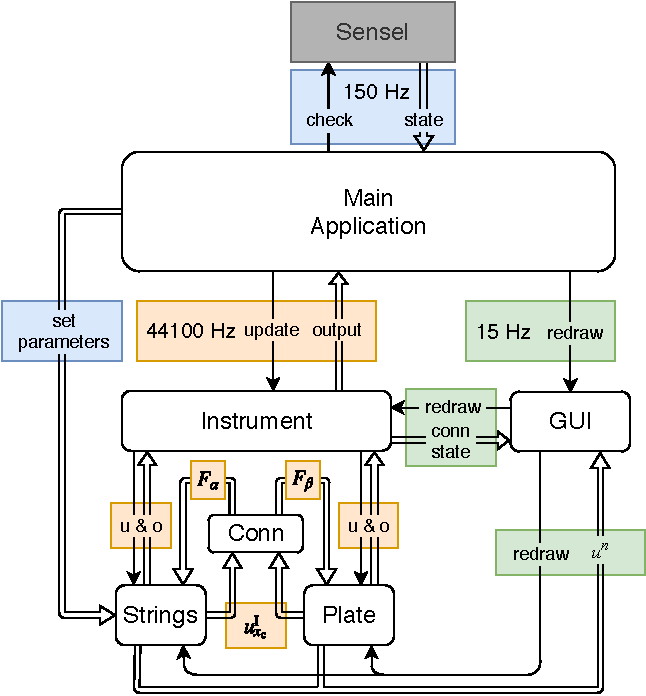
\includegraphics[width=\paperFigWidth\textwidth]{figures/JUCE.pdf}
\caption{System architecture flowchart. See Section \ref{sec:systemArch} for a thorough explanation. \label{fig:flowchart}}
\end{figure}

\subsection{System Architecture} \label{sec:systemArch}
The system architecture can be seen in Figure \ref{fig:flowchart}. The top box denotes the Sensel Morph (described in more detail in the next section) controlling the application, and the white boxes show the different classes or components of the application. The black arrows indicate instructions that one class can give to another and the hollow arrows show data flows between classes. All arrows are accompanied by a coloured box indicating which thread the instruction / dataflow is associated with and at what rate this thread runs.

The lowest priority thread, the graphics-thread, is shown by green boxes and runs at 15 Hz. This draws the states of the strings, connections and the plate on the screen.

Checking and retrieving the Sensel state happens at a rate of 150 Hz and is denoted by blue boxes. The parameters that the user controls by means of the Sensel, such as bowing position, force and velocity, will be updated in the models at this rate as well.

The highest priority thread is the audio-thread and runs at commonly-used sample rate 44,100 Hz. The main application gives an `update' (u) instruction to the instrument, which in turn updates the FDSs in its strings and plate. After the FDS update is done, the intermediate state at the connection points $u^\text{I}_{x_\text{c}}$ (where $x_\text{c} = l_{\text{c},\alpha}$ for the string or $x_\text{c} = (l_{\text{c},\beta}, m_{\text{c},\beta})$ for the plate) are sent to the connection (Conn) class which calculates the force-functions $F_\alpha$ and $F_\beta$. These values are then sent back to the string and plate classes and added to their respective states after which their outputs (o) (at arbitrary points) are sent back to the main application. See Algorithm \ref{alg:calcOrder} for this `order of calculation'.
% The most important thing in real-time implementation of FDSs, is to optimise the FDSs themselves as these will be ran at sampling rate. We make sure to only have one multiplication per location of $u$ per time step ($u_l^n$, $u_{l+1}^{n-1}$ etc) (\textbf{SEE APPENDIX DAFX PAPER}) %<-- needs to be more clear
% Furthermore, it is important to take note of is the order of calculation. First the non-extended schemes (Equations \eqref{eq:stiffString} and \eqref{eq:platePDE}) must be calculated before adding the effects of excitations (including bowing), which - in turn - needs to be calculated before adding the effects of connections (see Algorithm \ref{alg:calcOrder}).
\begin{algorithm}[h]
\fbox{\parbox{0.93\linewidth}{
    \While{application runs}{
    \For{all elements}{
    calculate intermediate state $\mathbf{u}^\text{I}$ using previous state values (as in Equation \eqref{eq:FDSform})
    
    $\quad \mathbf{u}^\text{I}_\text{s} = 2\mathbf{u}^n - \mathbf{u}^{n-1} + K\mathbfcal{F}$
    }
    \If{element is excited/bowed}{
    calculate excitation term $\mathbf{E}$ and add to intermediate state of the element
    
    $\quad \mathbf{u}^\text{I}_\text{s+e} = \mathbf{u}_\text{s}^\text{I} + \mathbf{E}$
    }
    \For{all connections}{
    calculate connection forces and add connection term $\mathbf{C}$ to elements to obtain the state at the next time step
    
    $\quad \mathbf{u}^{n+1}_\text{s+e+c} = \mathbf{u}_\text{s+e}^\text{I} + \mathbf{C}$
    }
    
    update state vectors
    
    $\quad \mathbf{u}^{n-1} = \mathbf{u}^n$
    
    $\quad \mathbf{u}^n = \mathbf{u}^{n+1}_\text{s+e+c}$
    
    
    increment time step
    
    $\quad n$++

    }
    }}
    \vspace{1em}
    \caption{Pseudocode showing the correct order of calculation. The subscripts for state vector $\mathbf{u}$ shows what it consists of (`s' for previous state, `e' for excitation and `c' for connection).\label{alg:calcOrder}}
\end{algorithm}

\section{Instruments and User Interaction}\label{sec:instruments}
In this section, the Sensel Morph (or simply Sensel) and user interface will be described in more detail. Furthermore, several configurations of strings, plates and connections that are inspired by real-life instruments will be presented. A demonstration of one of the instruments can be found in \cite{video}.

\subsection{Sensel Morph}
The Sensel Morph is a highly accurate touch controller that senses position and force of objects \cite{sensel2018} (see Figure \ref{fig:sensel}). We use the Sensel as an expressive interface for interacting with the instrument configurations. Right above the touch-sensitive area, the Sensel contains an array of 24 LEDs that can be controlled from the application.
\begin{figure}[ht]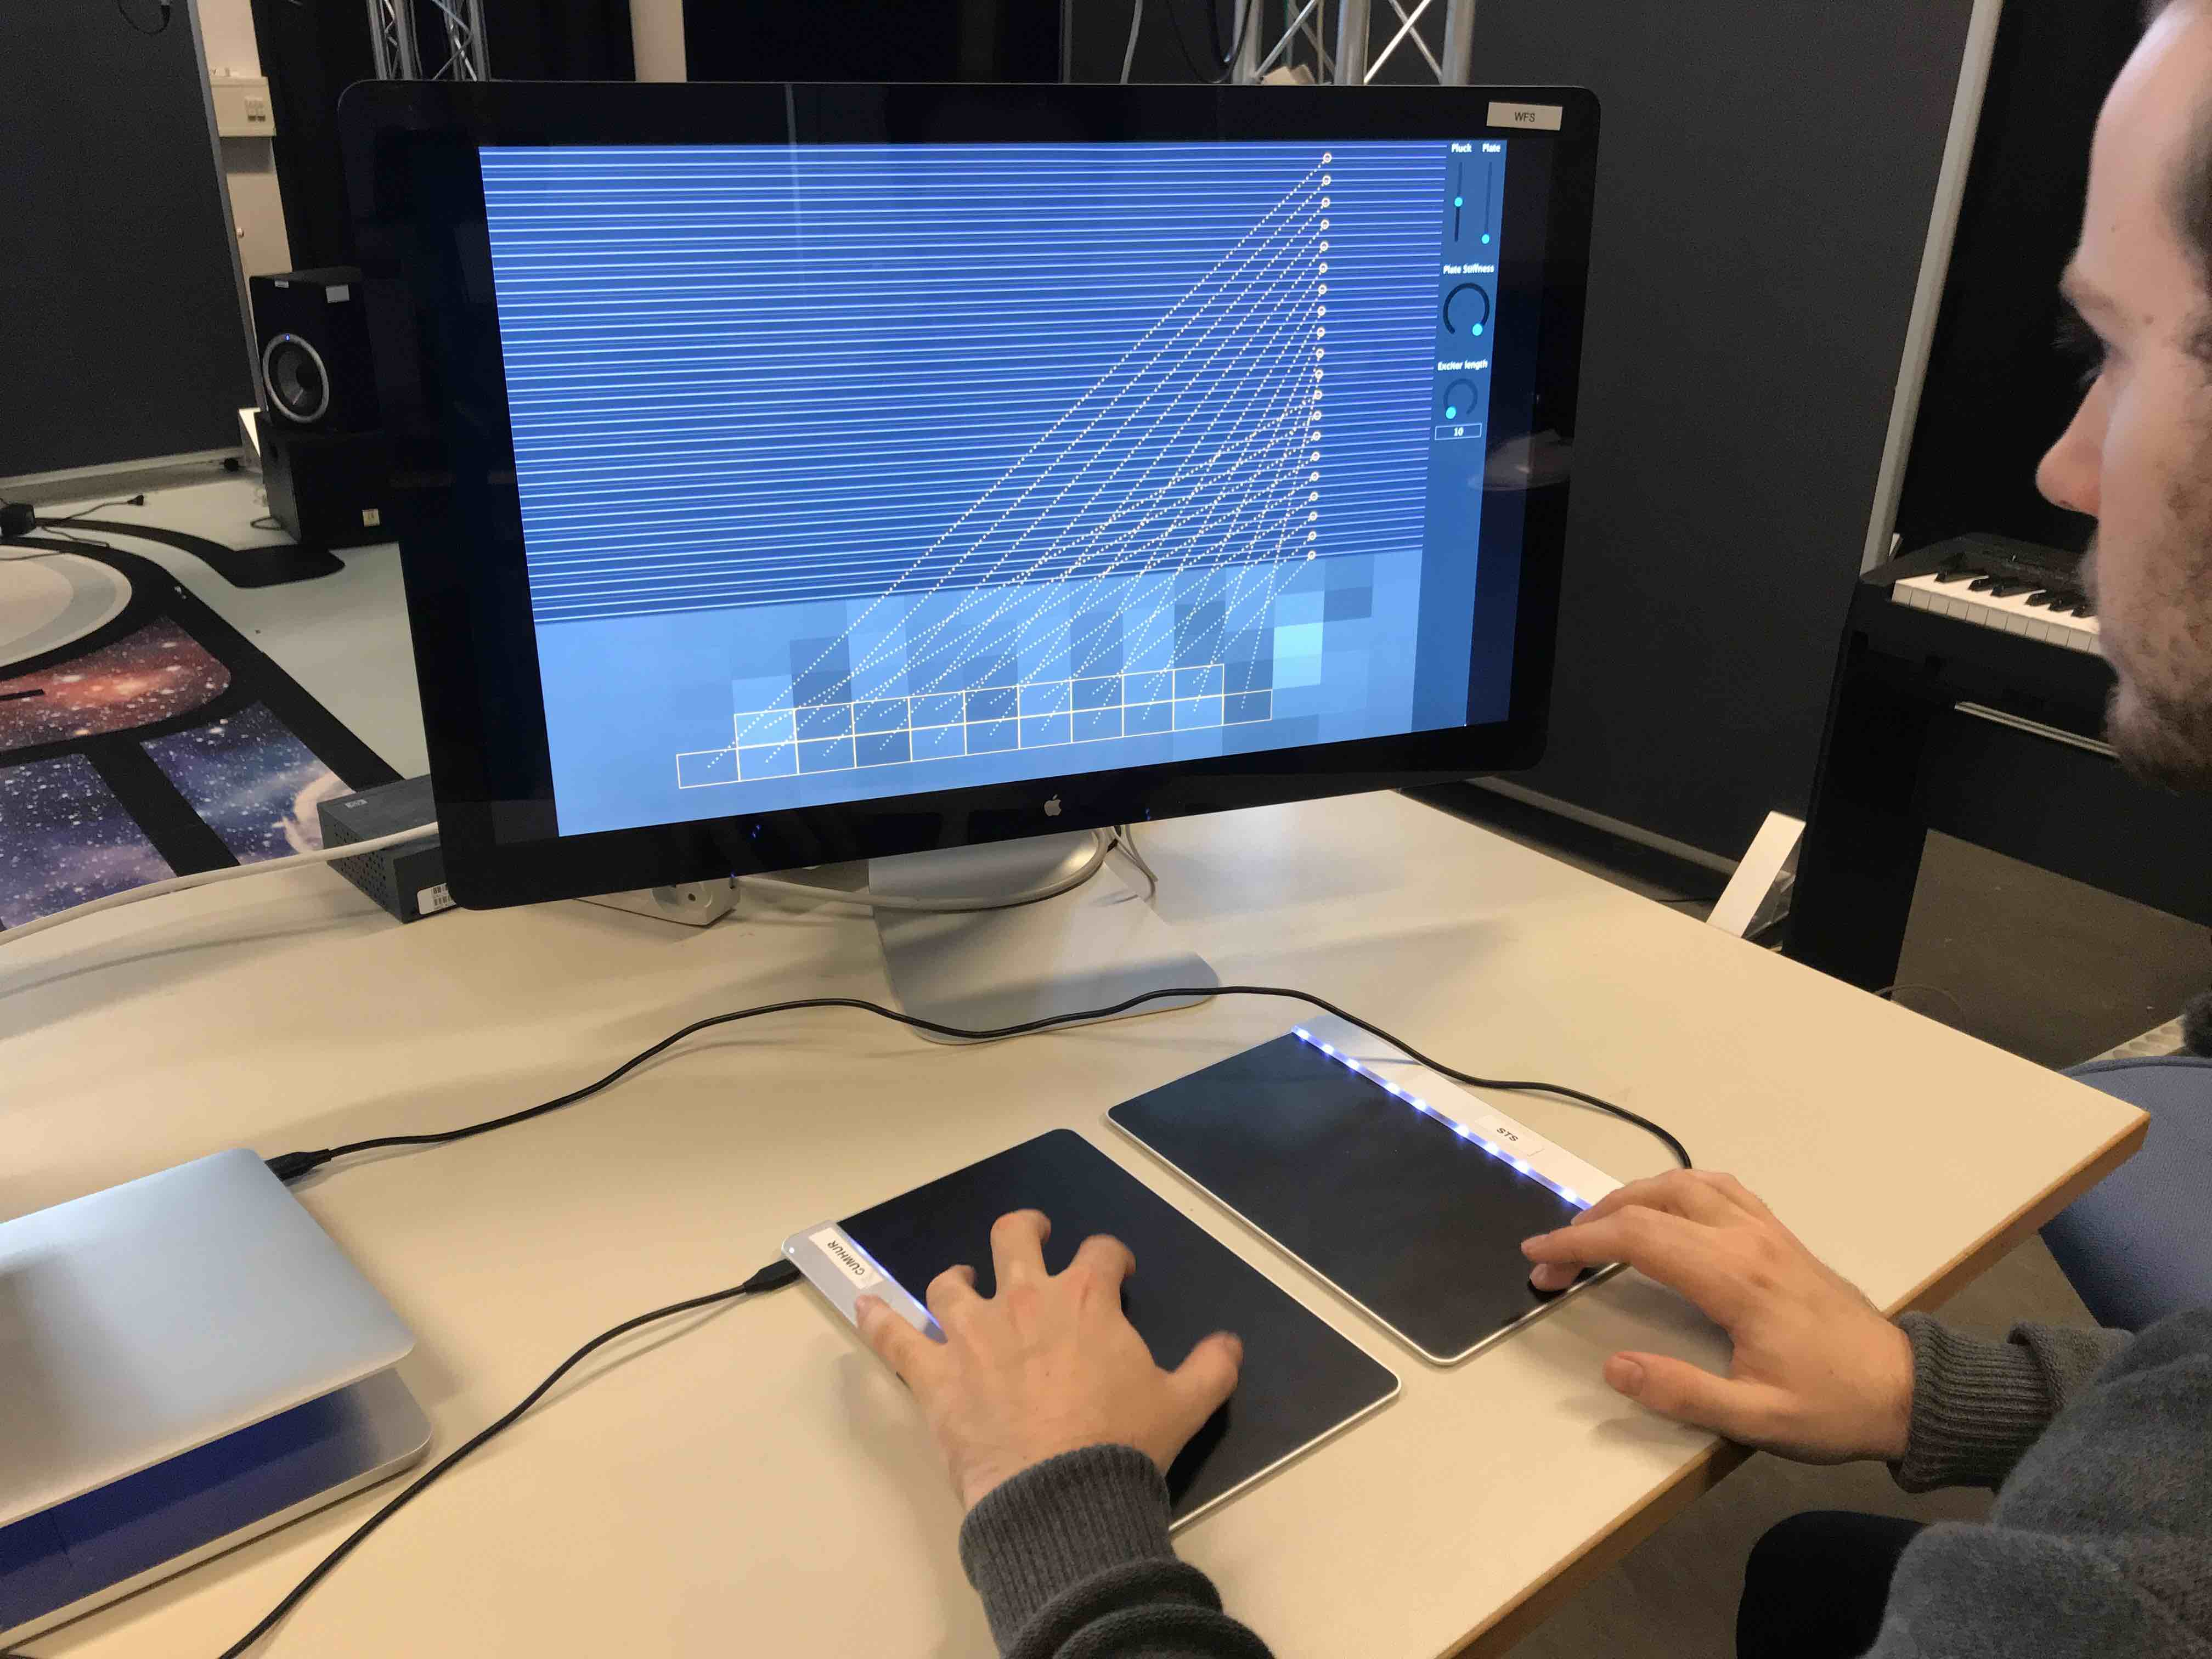
\includegraphics[width=\paperFigWidth\textwidth]{figures/senselLQ.jpg}\centering
\caption{Player using the Sensel Morphs to interact with one of the instruments.\label{fig:sensel}}
\end{figure}
% \subsubsection{Mapping strategies}
% Something about the different prototype mappings, and the "final" mapping 
% Lights to indicate bowing position or string position   
% % STEFANIA: add a pictue when we can see one person %interacting with the sensei and we see also the computer's %screen.
\subsection{User interface}
Strings are shown as coloured paths (see Figure \ref{fig:bowedSitar} for a descriptive visualisation). The state $\mathbf{u}^n$ of the string is visualised using the vertical displacement of the paths. Bowed strings are shown in cyan on the top left. The bow is shown as a yellow rectangle and moves on interaction. The fretting position is shown as a yellow circle. Plucked strings are shown in purple in the top right, underneath which the sympathetic strings are shown in light green. The plate is shown in the bottom using a grid of rectangles (clamped grid points are not shown). Its state is visualised using a grey-scale. Furthermore, connections are shown using orange circles/squares for the points of connection and dotted lines between these points. Lastly, all parameters that are controlled by the mouse such as output-level and plate-stiffness are located in a column on the right side of the application.

\subsection{Instruments}
We subdivide string-elements into three types: bowed, plucked and sympathetic strings. All strings will be connected to one plate acting as an instrument body of which the user can control the plate-stiffness. Furthermore, the user can change the output-level of each element type. Apart from these parameters, which are controlled by the mouse, the instruments are fully controlled by two Sensels. The instruments we have chosen as our inspiration are the sitar, the hammered dulcimer and the hurdy gurdy.

\subsubsection{Bowed Sitar}
The sitar is originally an Indian string instrument that has both fretted strings and sympathetic strings. Instead of plucking the fretted strings, we extended the model to bow them. Our implementation consists of 2 bowed strings (tuned to A3 and E4), 13 sympathetic strings (tuned according to \cite{sitarTuning}) and 5 plucked strings (tuned A3-E4 following an A-major scale) as it is also possible to strum the sympathetic strings. See Figure \ref{fig:bowedSitar} for a visual of the implementation. One Sensel is vertically subdivided into two sections; one for each bowed string. The first finger registered by the Sensel is mapped to a bow and the second is mapped to a fretting finger controlling pitch. The horizontal position of both fingers is visualised using the Sensel's LED array. The frets are not implemented as such (the pitch is continuous), but they are visualised for reference. The horizontal position of the first finger is mapped to the bowing position on the string, the vertical velocity to the bow velocity $v_\text{B}$ and the finger force is linked to the excitation function $F_\text{B}$ (both in Equation \eqref{eq:bowedString}). The other Sensel is subdivided into 5 sections mapped to the plucked strings. These sections are visualised by the LED array for reference.

The mass ratio for the bowed/plucked string to plate connections has been set to $\mathcal{M} = 2$ and ratio for the sympathetic string to plate connections has been set to $\mathcal{M} = 0.5$ to increase the effect that the playable strings have on the sympathetic strings.

\begin{figure}[h]
\centering
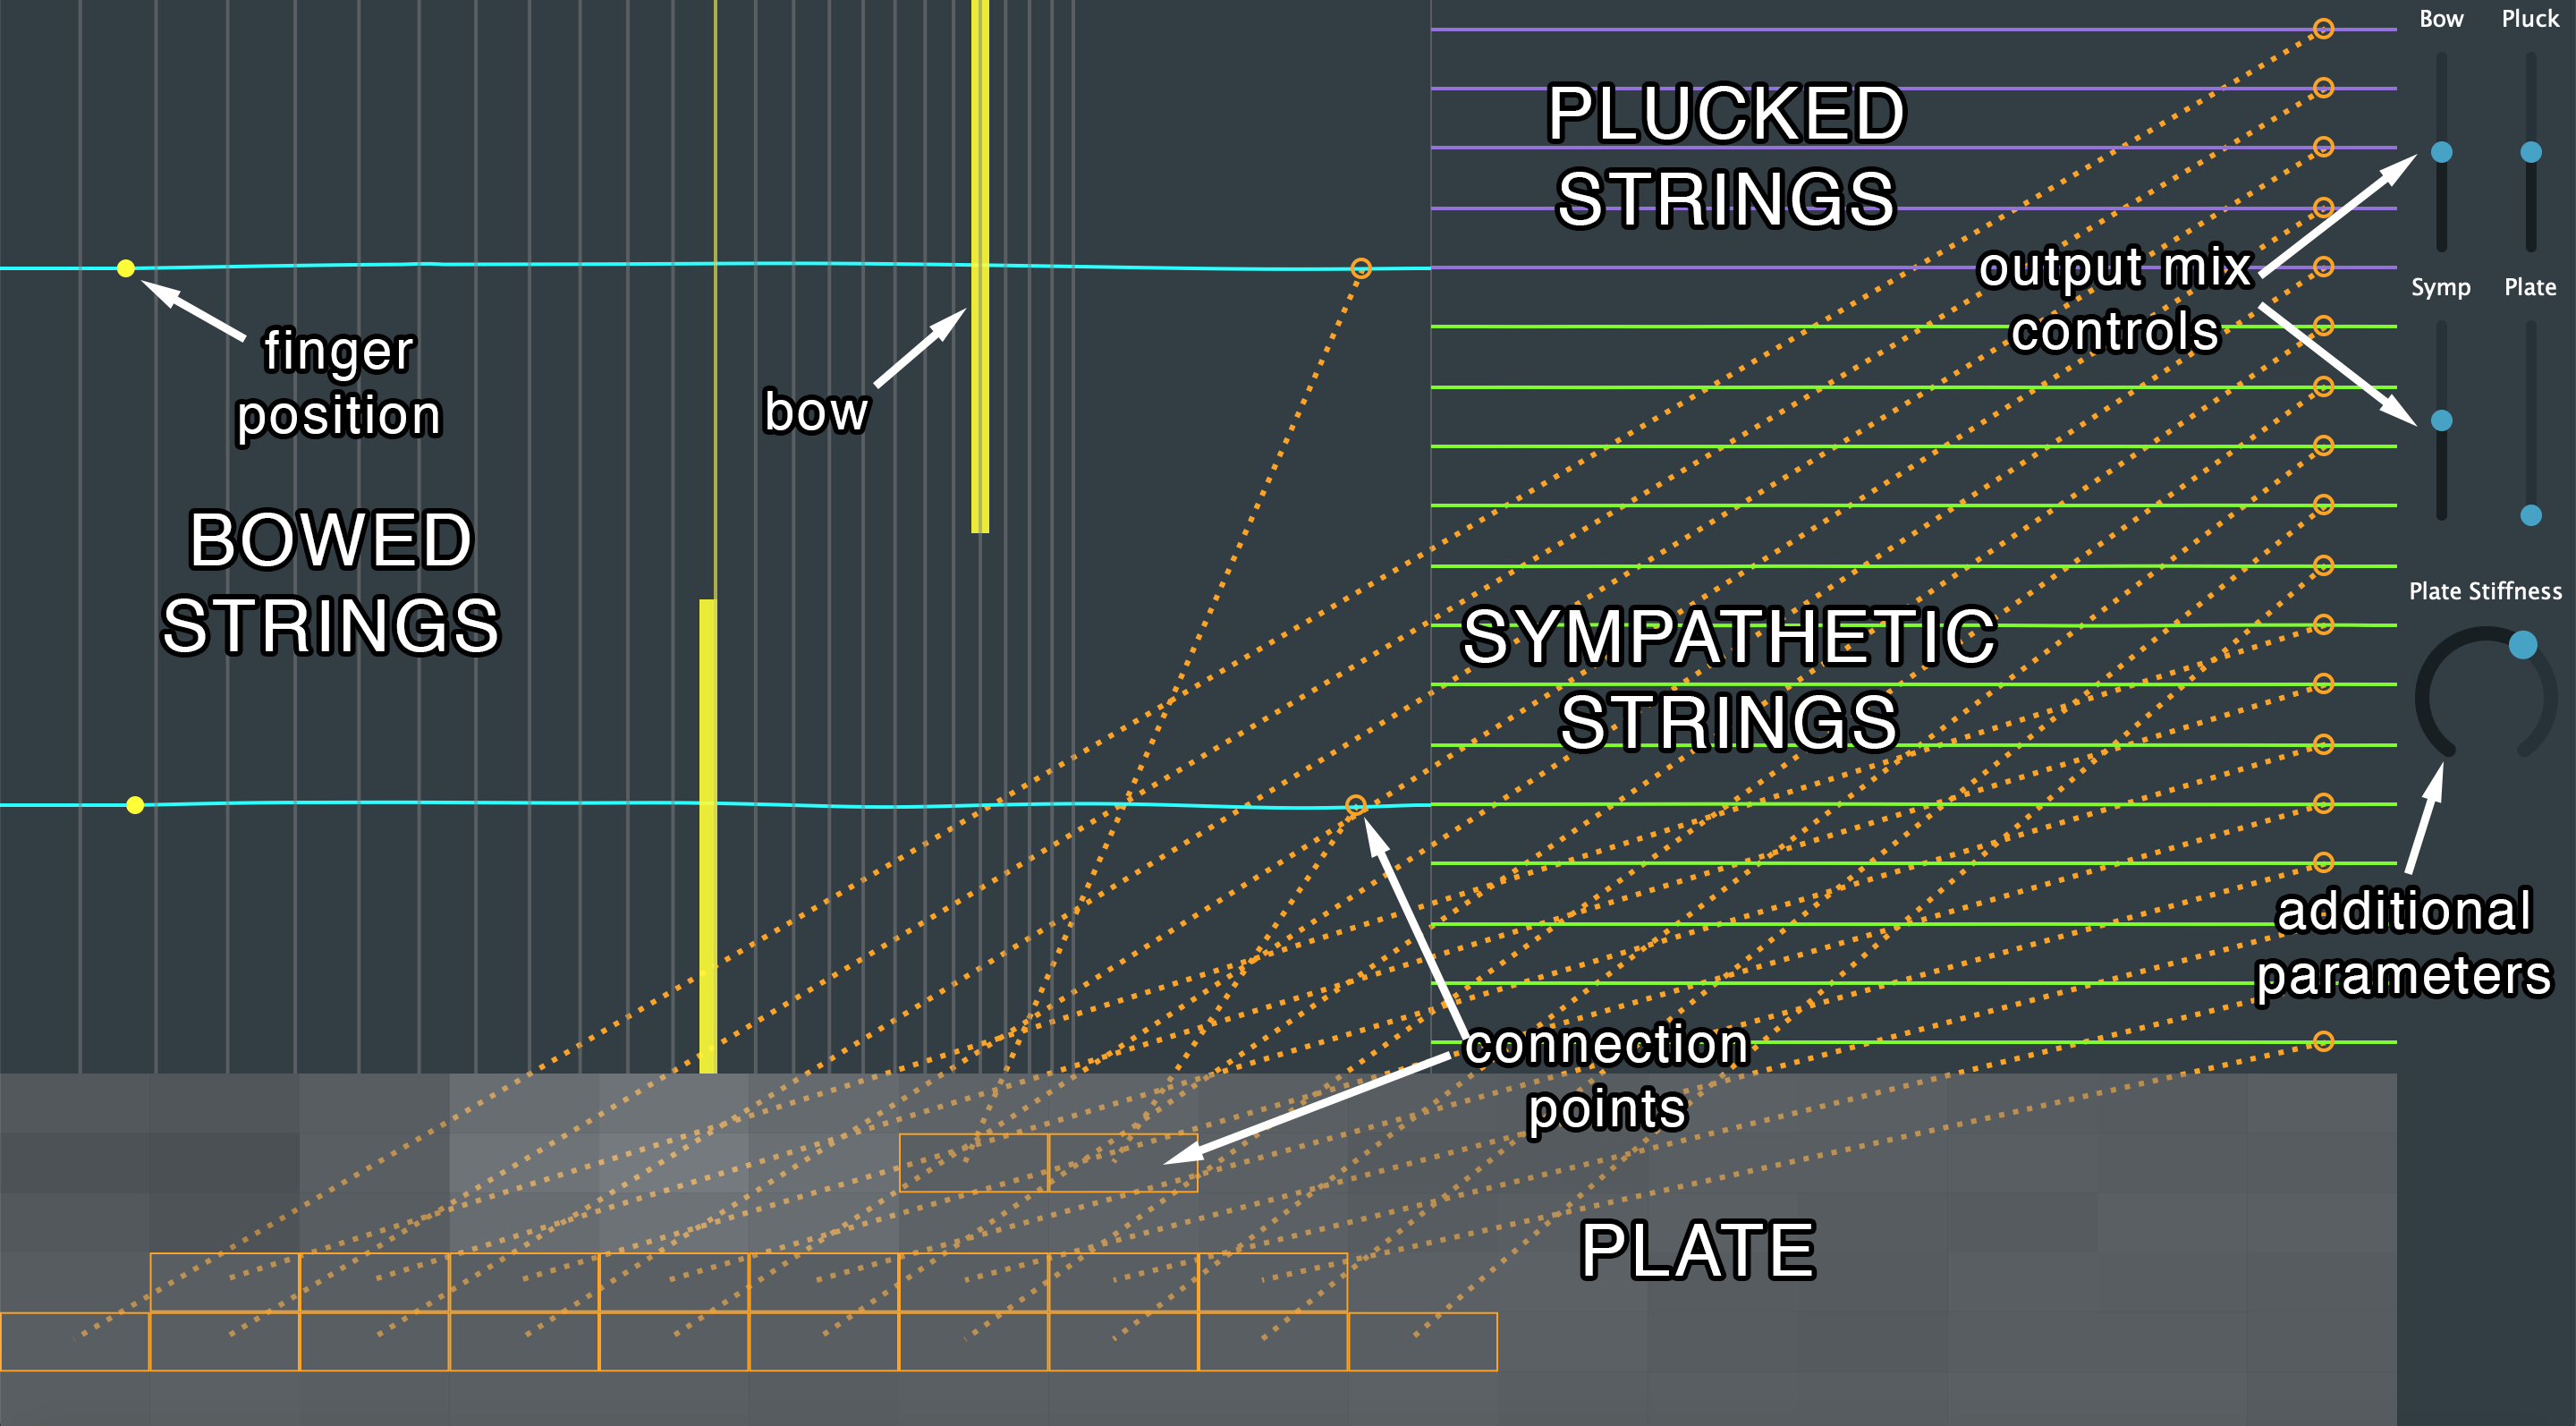
\includegraphics[width=\paperFigWidth\textwidth]{figures/BowedSitar.png}
\caption{The bowed sitar application. The descriptions of the different elements and other objects are shown in the image, but will (naturally) not be visible in the application. \label{fig:bowedSitar}}
\end{figure}

\subsubsection{Hammered Dulcimer}
The hammered dulcimer is an instrument that can be seen as an `open piano' where the musician has the hammers in their hand. Just like the piano, the strings are grouped in pairs or triplets
that are played simultaneously. 
In our implementation, we have 20 pairs of plucked strings. Even though most hammered dulcimers have more strings, we decided that this configuration has the highest number of strings while maintaining playability. One of each pair is connected to the plate which slightly detunes it, creating a desired `chorusing' effect. See Figure \ref{fig:dulcimer} for a visual of the implementation. In order for the excitation to more resemble a strike of a hammer than a pluck, the contents of the cosine in \eqref{eq:discExcitation} will be multiplied by 2 for the excitation to have a less abrupt ending, something desired for a hammered interaction. Moreover, the excitation-length can be changed to simulate short and long hammer-times.

The Sensels are placed vertically next to each other (see Figure \ref{fig:sensel}). The pair with the lowest frequency will then be located in the bottom right and the highest in the top left, as in the real instrument. As with the plucked strings of the bowed sitar, the LED array is used to visualise the way that the Sensel is subdivided, which is especially useful here as one Sensel controls 10 string-pairs. 

The mass ratio is set relatively high ($\mathcal{M} = 100$) to amplify the non-linear interaction between the strings and the detuning of the strings connected to the plate. 

\begin{figure}[h]
\centering
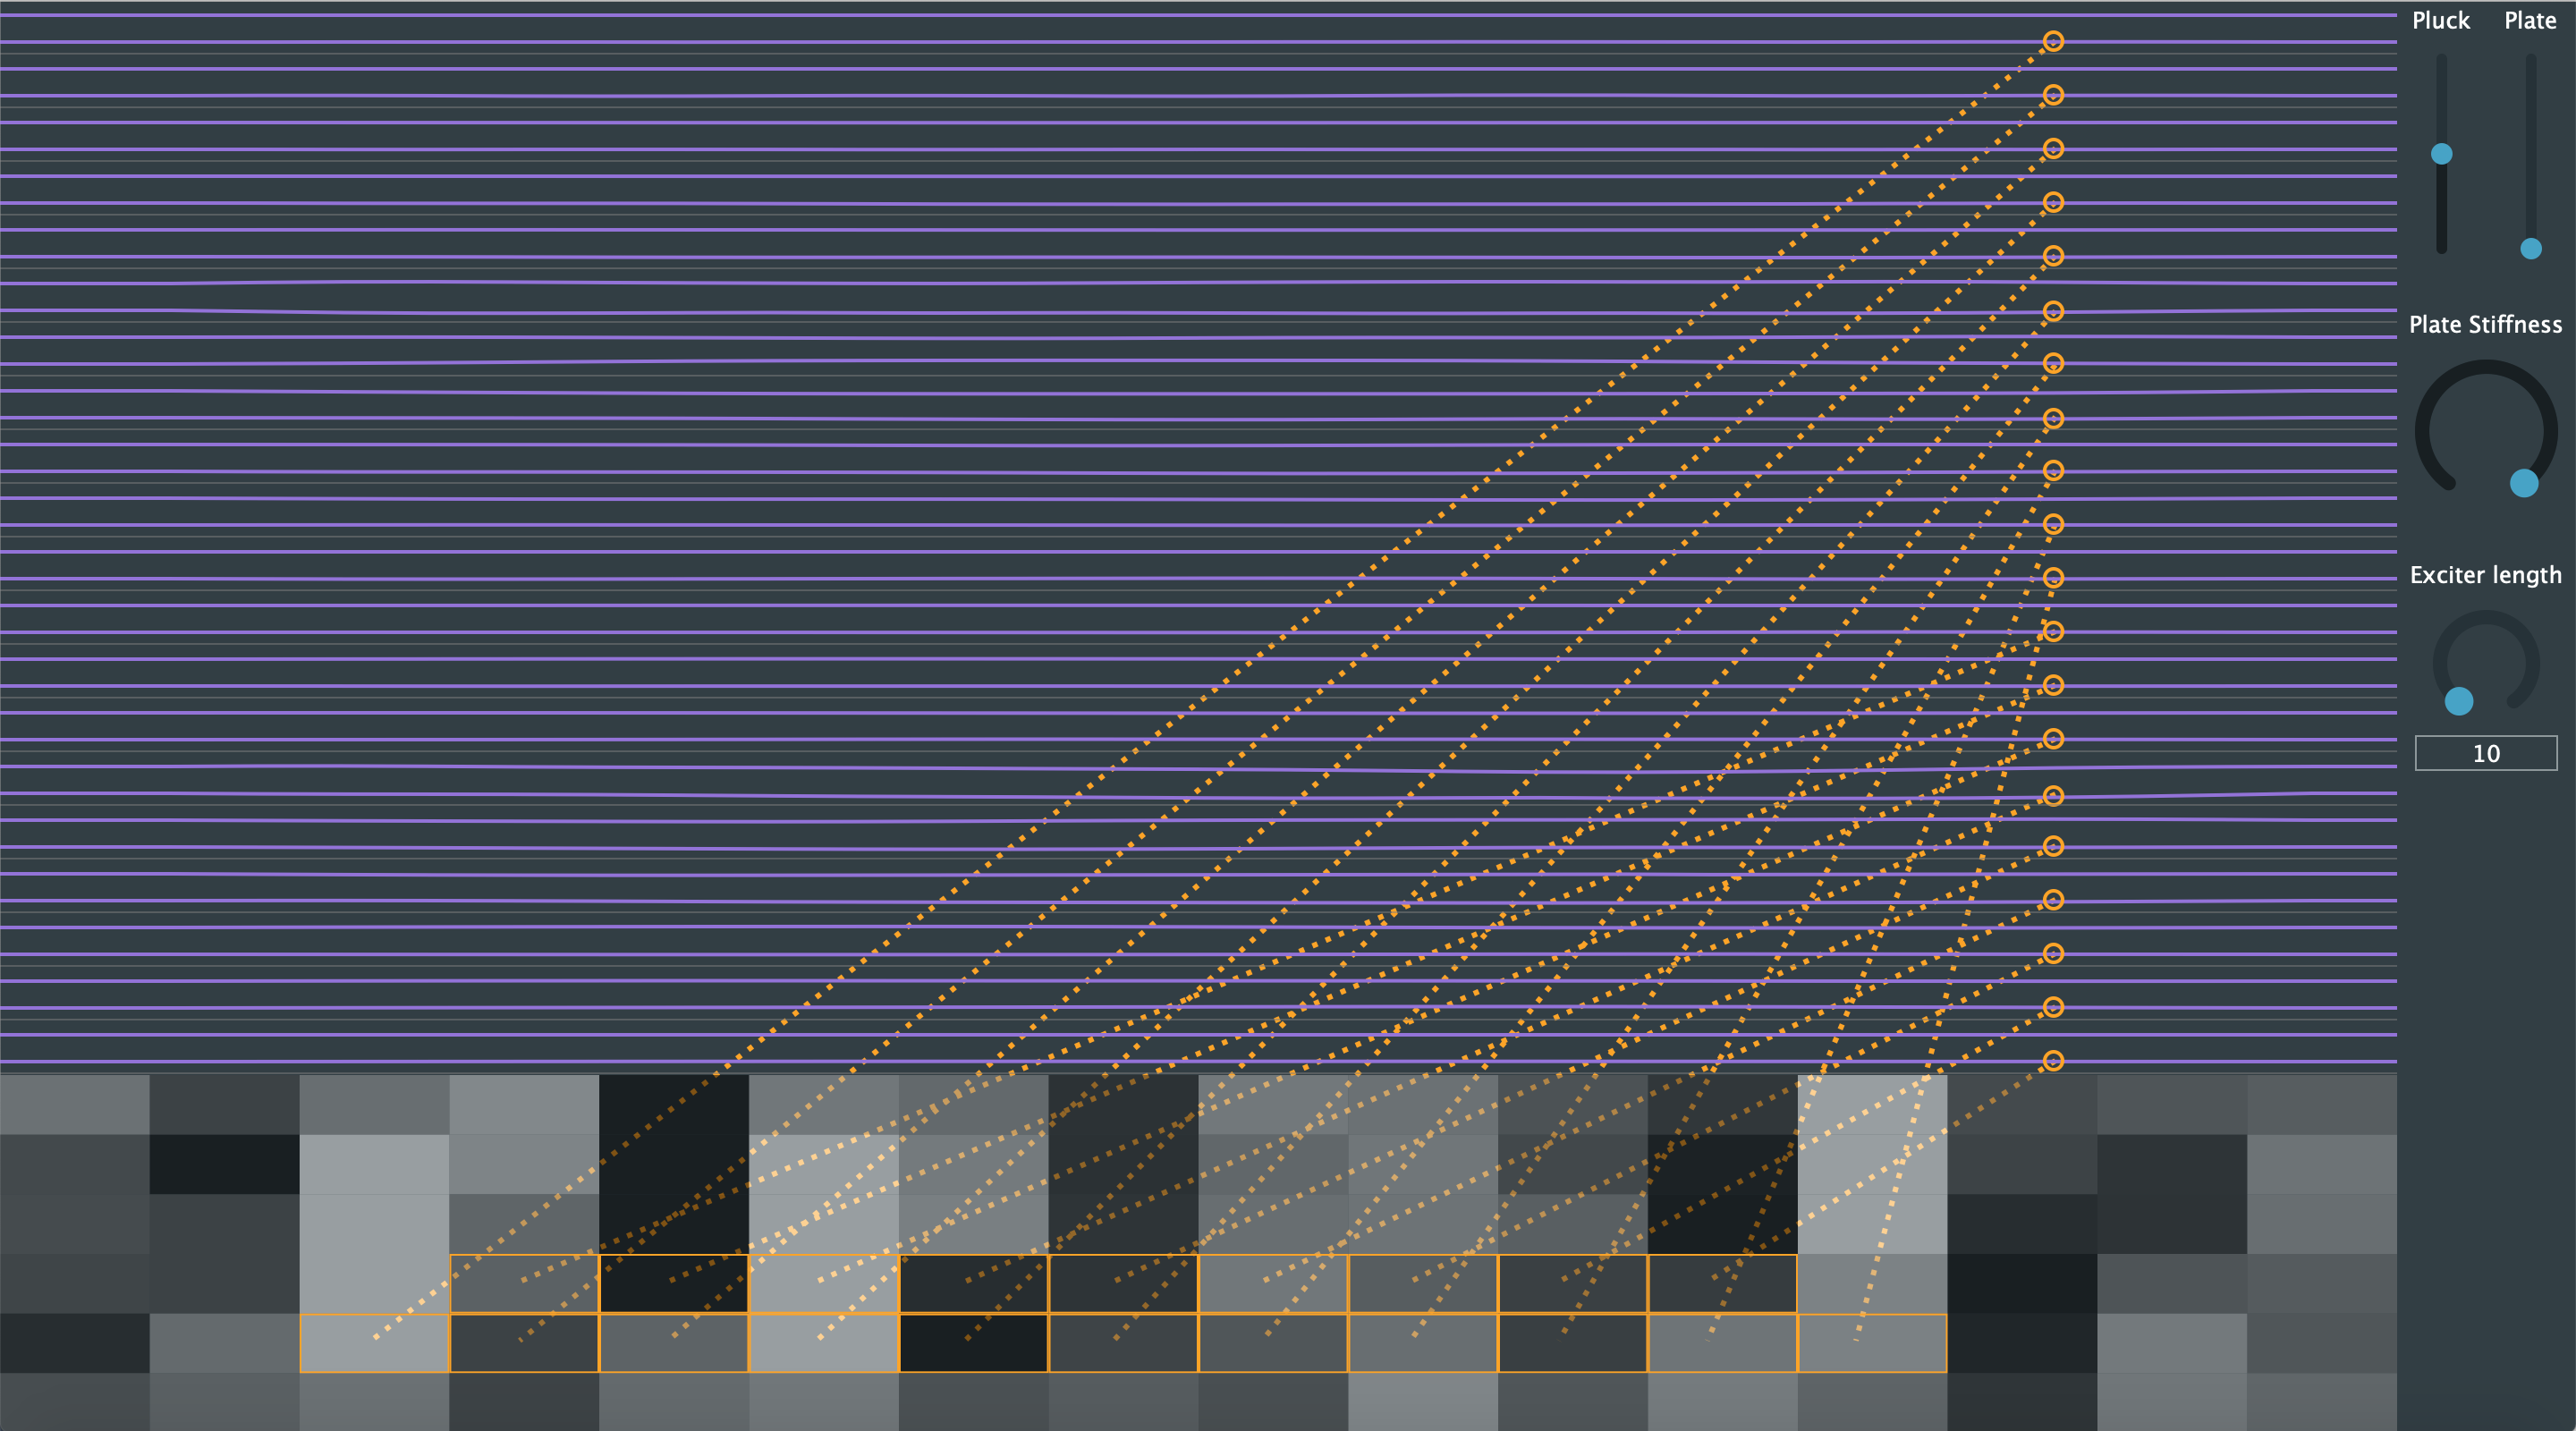
\includegraphics[width=\paperFigWidth\textwidth]{figures/dulcimer.png}
\caption{The hammered dulcimer application. \label{fig:dulcimer}}
\end{figure}

\subsubsection{Hurdy Gurdy}
The hurdy gurdy is an instrument that consists of bowed and sympathetic strings. The bowing happens through a rosined wheel attached to a crank and bows these strings as the crank is turned. It is possible to change the pitch of a few bowed strings - the melody strings - using buttons that press tangent pins on the strings at different positions. The other strings, referred to as drone strings, are mostly tuned lower than the melody strings and provide the bass frequencies of the instrument. The musician can place the bowed strings on rests that keep the wheel from interacting with it. 

Our implementation consists of 5 bowed strings subdivided into 2 drone strings tuned to A2, E3 and 3 melody strings tuned to A3, E4 and A4 and 13 sympathetic strings tuned the same way as the sympathetic strings in bowed sitar. Furthermore, the mass ratios have been set the same as in the bowed sitar application. See Figure \ref{fig:hurdyGurdy} for a visual of the implementation.

The Sensel is vertically subdivided into 5 rows that control whether the strings are placed on the wheel. The bowing velocity is mapped to the average pressure of the fingers. The fundamental frequency (in the model $\gamma / 2$) of the melody-strings is changed by a Sensel with a piano-overlay acting as a midi controller. A demonstration of this instrument can be found in \cite{video}. It is interesting to note here that the sympathetic strings that are in tune with the harmonics of the bowed strings resonate most, which is expected to happen in the real world as well.

\begin{figure}[h]
\centering
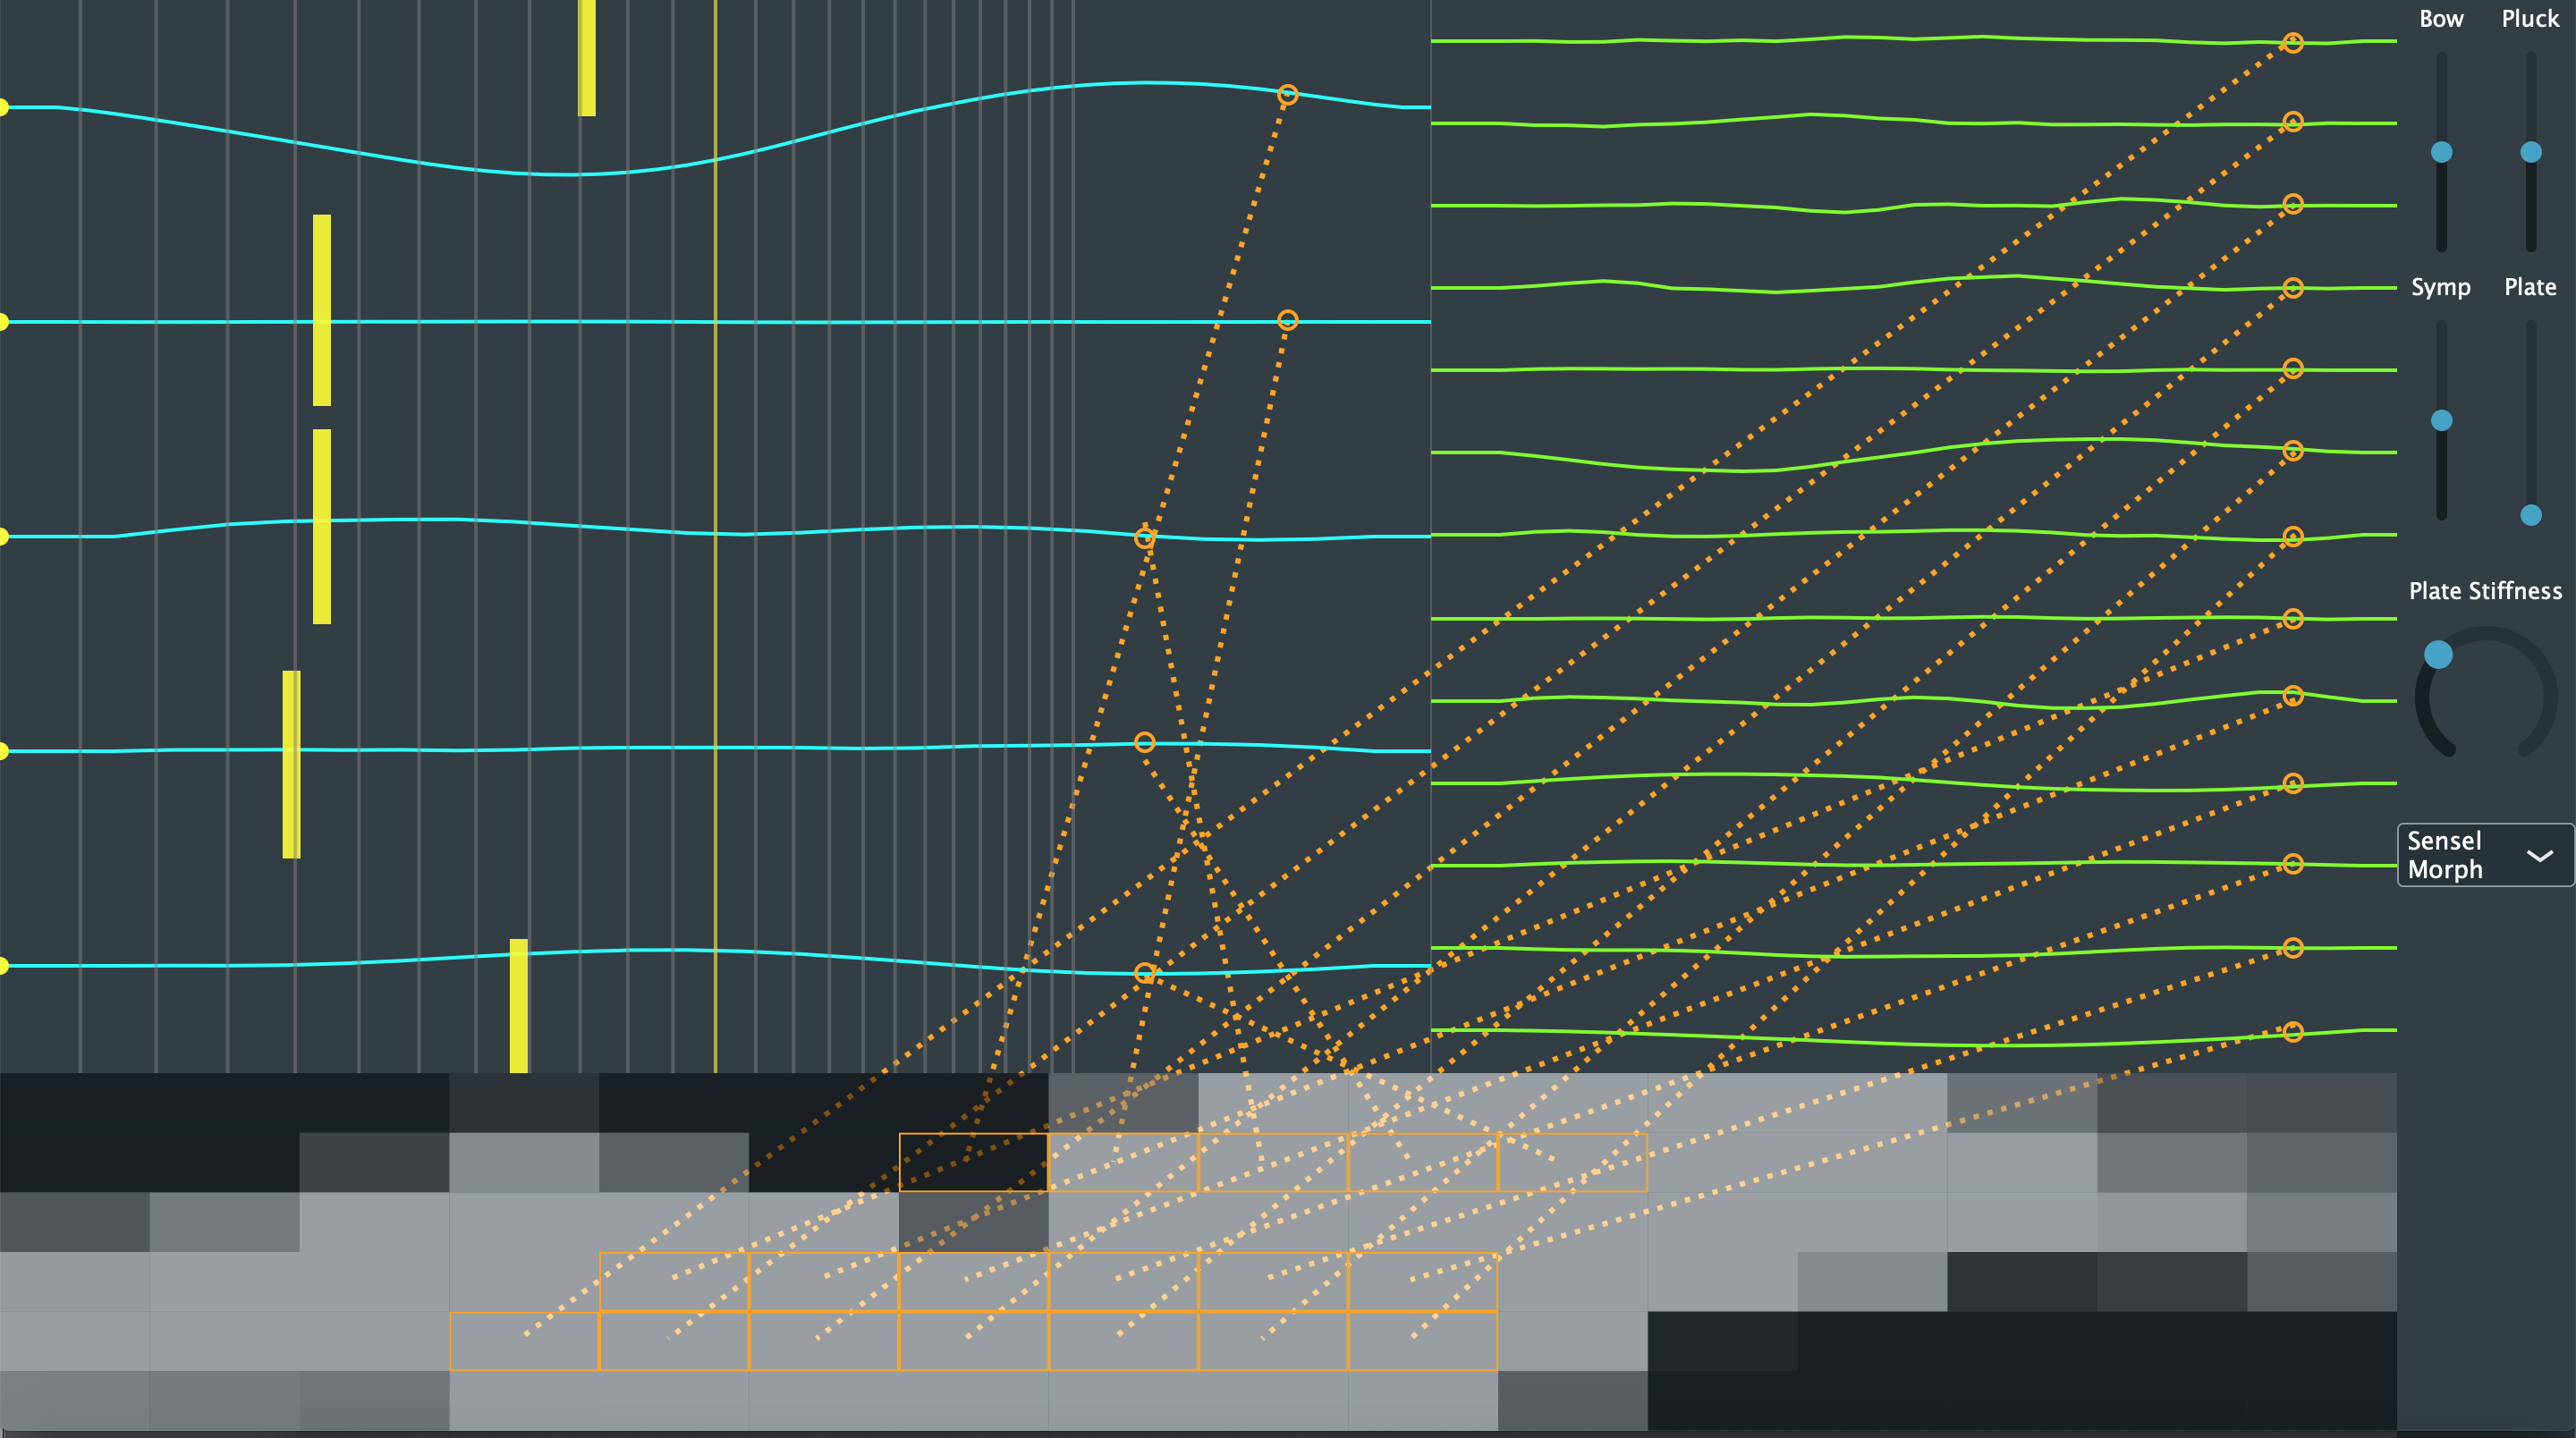
\includegraphics[width=\paperFigWidth\textwidth]{figures/HurdyGurdy.png}
\caption{The hurdy gurdy application. \label{fig:hurdyGurdy}}
\end{figure}

\section{Results and Discussion}\label{sec:discussion}
Table \ref{tab:CPU} shows the CPU usage (on the same MacBook Pro 2.2 GHz i7 as described before) for the three instruments presented in the previous section. As the Sensel thread contributes a negligible amount to the CPU usage, this is not shown in the table.

\begin{table}[h]
\centering
\begin{tabular}{|c|c|c|c|}
\hline
Application & No Sound & No Graphics & Total \\
\hline
Bowed Sitar &32 &63 &85 \\
Dulcimer &30 &66 &85 \\
Hurdy Gurdy &28 &58 &78 \\
\hline
\end{tabular}\caption{CPU usage (in \%) for the instruments found in Section \ref{sec:instruments}. Values show usage of one (virtual) thread and have been taken as an average (with a margin of \textapprox5\%) over a short period of time. The two middle columns show usage when the sound or graphics thread has been turned off.}\label{tab:CPU}
\end{table}

\noindent As can be seen from the table, all instruments use about the same amount of CPU and none of them have audible dropouts (CPU $<$ 100\%). It can be observed that the graphics use about 20\% of the CPU, indicating that there is still much room to increase the complexity of the instrument-configurations before dropouts will occur. On the other hand, should the instruments be used in parallel with other audio applications or plug-ins, the CPU usage has to be greatly reduced. The first step towards this would be to vectorise the FDSs using AVX instructions.

While our instruments have been not formally evaluated yet, we have performed some qualitative evaluations with sound and music computing experts. The goals of the evaluations were to explore the playability of the instrument, sonic quality and intuitiveness of control. These evaluations showed that especially the bowing interaction feels intuitive and creates a natural sound. The overall sound of the instruments was generally judged to be interesting, but not ``sounding like a real-life instrument". This makes sense, as we did not seek to perfectly model each instrument, but rather used them as an inspiration for the configurations of the physical models. The next step for sound quality would be to replace the thin plate with a more realistic element, such as a wooden instrument body.

% We did an informal test with a lecturer of the Rytmisk Center K{\o}benhavn 
% The interaction with the bow has been found very natural. Bow force and velocity... 

\section{Conclusion}\label{sec:conclusion}
% In this paper, we presented several instruments consisting of physical models of bowed and plucked strings, plates and connections between them. These instruments have been successfully implemented in real-time and are controlled by a pair of Sensel Morphs. The interaction has been found natural and the output sound interesting. As mentioned, the first steps to improve this project are to optimise the algorithm using AVX vector instructions and to replace the plate with a more realistic (wooden) instrument body.

In this paper, a real-time modular physical modelling synthesis environment structured as a network of connected strings and plates has been presented. Several instruments have been created in the context of this environment which can be played by a pair of Sensel Morphs allowing for highly expressive control of these instruments. Informal evaluations with professional musicians have confirmed that the interaction is found natural and the output sound interesting. Further steps to improve this project are to optimise the algorithm and to replace the plate with a more realistic instrument body.
\section{Acknowledgments}
This work is supported by NordForsk's Nordic
University Hub Nordic Sound and Music Computing Network
NordicSMC, project number 86892.
